\documentclass[11pt]{article}
\usepackage[T1]{fontenc}
\usepackage[utf8]{inputenc}
\usepackage{lmodern,microtype}
\usepackage[a4paper,margin=28mm]{geometry}
\usepackage{amsmath,amssymb,amsthm,booktabs,tabularx,longtable,graphicx}
\usepackage{tikz}
\usetikzlibrary{positioning,arrows.meta}
\usepackage[hidelinks]{hyperref}
\usepackage[round]{natbib}
\newtheorem{remark}{Remark}[section]
\newcommand{\code}[1]{\texttt{\detokenize{#1}}}
\newcommand{\Warning}{\textbf{DRAFT --- NOT ACCEPTED}}
\tikzset{obj/.style={draw,rounded corners,minimum width=17mm,minimum height=8mm,align=center},
arr/.style={-{Latex[length=2mm]},thick}}

\title{Mathematical Closures in the Permansson Strategic--World Framework\\
\large Canonical Transport, Measurable Two-Player Recovery and Nonlinear Occupation}
\author{Marcus Hermansson\\Independent researcher}
\date{Working source draft --- 21 October 2026}
\begin{document}
\maketitle
\begin{center}\fbox{\parbox{0.9\textwidth}{\centering\Warning\\
This manuscript is the single-PR mathematical-closure working draft. Earlier
canonical and conditional proofs have compiled, but new final source-specific
P--04/P--05/P--06 bridges, original 45-case acceptance, full independent review
and paper-release approval remain unverified until final source-bound gates.}}\end{center}
\begin{abstract}
An explicitly scoped research and proof-integration programme connecting canonical strategic--world path laws to
original constitutive margins, recover arbitrary-measurable conditional-product
two-player models, and formalize a finite nonlinear occupation counterexample.
We separate historical proved providers from work in progress, preserve the
original typed strategic interventions and comparison domains, and distinguish
formal verification from empirical regime identification.
\end{abstract}
\tableofcontents
\section{Original typed semantics}
The original v0.1.8 framework \citep{PRT2026} defines the joint state
$Y=S\times X$, action selection $\alpha$, physical world transition $P$,
and strategic update $U$. Its induced Markov kernel has the ordered meaning
\[
K((s,x),d(s',x'))=
\int_A\alpha(da\mid s,x)\,P(dx'\mid s,x,a)\,
U(ds'\mid s,x,a,x').
\]
A strategic intervention changes an admissible strategic mechanism while
preserving the physical $P$ \emph{within the model}. Generated Regimes
require their separately certified ex-ante persistence, descriptor and
occupation semantics. A Permansson Regime additionally requires original
strategic constitution on the certified comparison set.
\begin{figure}[htbp]\centering
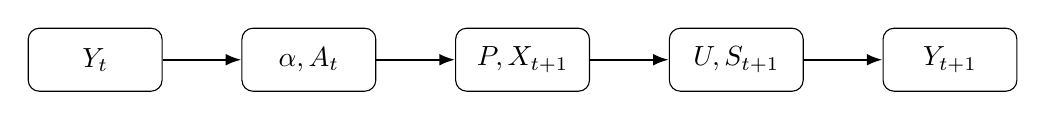
\begin{tikzpicture}[node distance=10mm]
\node[obj] (y) {$Y_t$}; \node[obj,right=of y] (a) {$\alpha,A_t$};
\node[obj,right=of a] (p) {$P,X_{t+1}$};
\node[obj,right=of p] (u) {$U,S_{t+1}$};
\node[obj,right=of u] (z) {$Y_{t+1}$};
\draw[arr] (y)--(a);\draw[arr] (a)--(p);
\draw[arr] (p)--(u);\draw[arr] (u)--(z);
\end{tikzpicture}
\caption{The actual $\alpha\to P\to U$ chronology; $P$ remains fixed
under admissible within-model strategic intervention.}
\end{figure}

\section{Source foundations: what already exists}
The historical v0.1.8 original core and source-reviewed PR79 research
library provide \code{inducedKernel}, \code{pathLaw},
\code{constitutiveMargin}, \code{HasConstitutiveOutputErrors}, the
dependent-history \code{evolution} and discounted projected-output
providers. Finite Markov C10/C11 work, canonical random occupation
laws, and solver certificates are separate existing proofs under their
actual finiteness, information and property hypotheses.
The historical 42-contract atlas and the full 45 acceptance conditions
are obligations and source evidence, not 45 automatically accepted claims.
\begin{remark}
An existing theorem proves exactly its stated source type and assumptions;
it does not imply an unrestricted generalization, a deployment safety
certificate, or identified empirical GR/PR status.
\end{remark}


\paragraph{Already integrated by PR \#112.}
Source-bound compiled providers include the actual canonical time-marginal
identity, full-path discounted property and \emph{conditional} original
margin bound, arbitrary-measurable conditional-product two-player induced
kernels and all-initial paths, plus the genuine native finite phase/world
kernel and original deterministic infinite path-law identity. The remaining
work concerns \emph{constructing} these conditional hypotheses for declared
source protocols and determining the true nonlinear occupation-limit values.

\section{P--04: Discounted output to original constitutive margin}
\textbf{Status: canonical marginal and conditional whole-path original-margin adapters exist; actual separate source-bound witnesses require final verification.}
The scoped theorem \code{canonical_nth_marginal_eq_evolution} concerns
the genuine canonical time-$n$ marginal, not the full property or a
closed original constitutive margin.
For typed compression $q:Y\to\bar Y$ and fixed $0\le\beta<1$, the original
whole-path score is $\Phi(w)=(1-\beta)\sum_{n\ge0}\beta^n g_n(w_n)$,
with fixed measurable $0\le g_n\le1$.
Baseline and intervention must each use their \emph{actual canonical law}.
The required chronological retained-mass envelope on every original
comparison start $y\in B_1$ is
\[
E_s(y)=\sum_{n\ge0}(1-\beta)\beta^n
\left(1-(1-\varepsilon_s(y))\prod_{t<n}(1-\eta_{s,t}(y))\right)
,\quad s\in\{0,J\}.
\]
Matched Dirac starts have $\varepsilon_s(y)=0$; a distinct general
initial-law result must retain possible nonzero $\varepsilon$.
Uniform $E_0\le e_0$ and $E_J\le e_J$ and the exact equality
$\bar B_1=q(B_1)$ are required for the original-margin conclusion
$|\kappa-\bar\kappa|\le e_0+e_J$, with any reporting errors $b_0,b_J$
recorded separately.
\begin{figure}[htbp]\centering
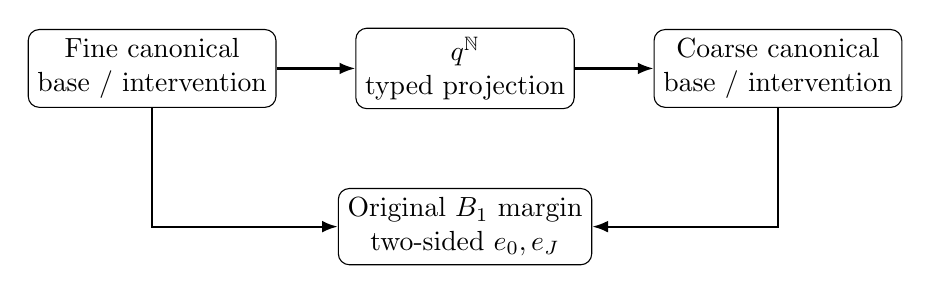
\begin{tikzpicture}[node distance=10mm]
\node[obj] (f) {Fine canonical\\base / intervention};
\node[obj,right=of f] (q) {$q^{\mathbb N}$\\typed projection};
\node[obj,right=of q] (g) {Coarse canonical\\base / intervention};
\node[obj,below=of q] (m) {Original $B_1$ margin\\two-sided $e_0,e_J$};
\draw[arr] (f)--(q);\draw[arr] (q)--(g);
\draw[arr] (f)|-(m);\draw[arr] (g)|-(m);
\end{tikzpicture}
\caption{Both baseline and intervention output laws must transport to
the original full-$B_1$ margin API; diagram is not a proof receipt.}
\end{figure}
A positive numerical margin does not by itself imply Exact GR/PR.


\paragraph{Source-specific witness.}
The final integration distinguishes the real baseline witness
$(K_0,\bar K_0,R_0,\eta_0)$ from the real treated witness
$(K_J,\bar K_J,R_J,\eta_J)$. Each subkernel must be dominated on all
required source states and its projected row must be dominated by the
proper \emph{coarse} kernel; neither is an assumed TV number. Each
point-initialized original comparison starts from its actual Dirac law,
so the initial mismatch vanishes only for that matching construction.
The two model-output bounds must then be used through the unchanged
original \texttt{HasConstitutiveOutputErrors} and full-$B_1$
\texttt{constitutiveMargin} API. Positive leakage still defeats an Exact
GR transfer regardless of how small the discounted error becomes.

\section{P--05: Measurable two-player reconstruction}
\textbf{Status: generic measurable kernel and canonical entire-path recovery compiled in prior PRs; concrete binary matched-intervention/original-margin closure is the final integration.}
The original strategic state is $S_0\times\prod_{i\in\mathrm{Fin}\,2}S_i$.
The binary target is $S_0\times(S_0^{\rm priv}\times S_1^{\rm priv})$,
with joint states formed by adjoining $X$. Distinct measurable maps
$\phi_S$, $\phi_A$, $\phi_Y$, $\phi_{\rm WorldInput}$ and
$\phi_{\rm UpdateInput}$ are mandatory. The update kernel outputs
strategic state $S$, not joint state $Y$, and must preserve separately
conditioned common/private updates:
\[
(\phi_S)_\#U_G(y,a,x')
=U_{\rm bin}(\phi_Y(y),\phi_A(a),x').
\]
Together with physical input pullback and action product mapping,
the target is $K_{\rm bin}\circ\phi_Y=(\phi_Y)_\#K_{\rm orig}$
on \emph{every measurable event}, then complete canonical path-law
transport for every initial law and both legal CL/OL intervention families.
\begin{figure}[htbp]\centering
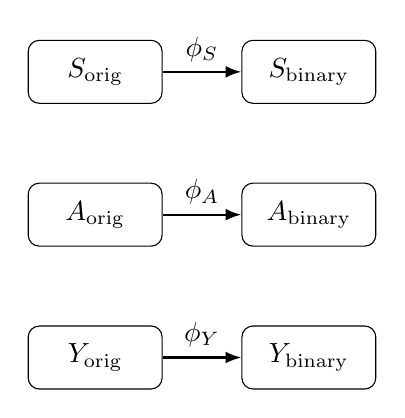
\begin{tikzpicture}[node distance=10mm]
\node[obj] (s) {$S_{\rm orig}$}; \node[obj,right=of s] (sb) {$S_{\rm binary}$};
\node[obj,below=of s] (a) {$A_{\rm orig}$};
\node[obj,right=of a] (ab) {$A_{\rm binary}$};
\node[obj,below=of a] (y) {$Y_{\rm orig}$};
\node[obj,right=of y] (yb) {$Y_{\rm binary}$};
\draw[arr] (s)--node[above] {$\phi_S$} (sb);
\draw[arr] (a)--node[above] {$\phi_A$} (ab);
\draw[arr] (y)--node[above] {$\phi_Y$} (yb);
\end{tikzpicture}
\caption{The update output uses $\phi_S$, not $\phi_Y$; inputs retain
both action and realized next-world state.}
\end{figure}
This concerns the declared conditional-product subclass only.


\paragraph{Admissible matched protocols.}
For each treated player $i\in\mathrm{Fin}\,2$, the binary counterpart is
constructed by applying the \emph{same} source closed-loop or admitted
open-loop source mechanism before reindexing. The original and binary
physical kernels remain separately fixed. This replaces the earlier
conditional \texttt{Jbar}/\texttt{hJ} input with real admitted binary
interventions and original all-measurable-event kernel intertwining.
Only the conditional-product subclass is included; hidden common
correlation is an excluded model class.

\section{P--06: Native strategic phase and nonlinear occupation}
\textbf{Status: native atoms under compilation; full occupation pending.}
One native strategic-world model uses phase memory $S=\mathrm{Fin}\,3$,
physical world $X=\mathrm{Bool}$, action $A=\mathrm{Bool}$ and the
\emph{same} primitives $P((p,x),a)=\delta_a$ and
$U((p,x),a,x')=\delta_{(p+1)\bmod3}$ under all compared controllers.
The phase-aware policy selects $a=(p\neq2)$ and from $(0,F)$ generates
$(0,F)\to(1,T)\to(2,T)\to(0,F)$.
\begin{figure}[htbp]\centering
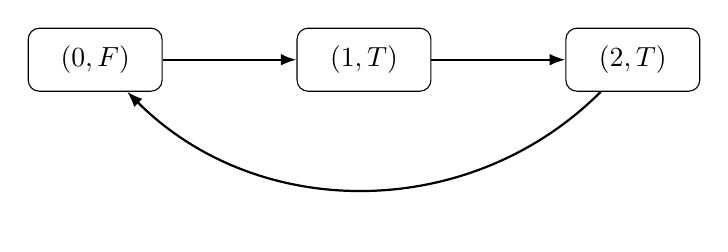
\begin{tikzpicture}[node distance=17mm]
\node[obj] (a) {$(0,F)$};\node[obj,right=of a] (b) {$(1,T)$};
\node[obj,right=of b] (c) {$(2,T)$};
\draw[arr] (a)--(b);\draw[arr] (b)--(c);
\draw[arr] (c) to[bend left=45] (a);
\end{tikzpicture}
\caption{The native three-phase cycle with projected Bool true mass $2/3$.}
\end{figure}
The proposed original nonlinear objective is the \emph{expectation}
of $F(\nu)=1-|\nu(\{T\})-2/3|$ evaluated on the genuine pathwise
empirical occupation-limit law, not $F$ of its barycenter.
The selected comparison is only over four deterministic \emph{phase-blind}
physical feedbacks $\pi:\mathrm{Bool}\to\mathrm{Bool}$; the proposed maximum
is $5/6$, versus $1$ for phase-aware policy. A stationary randomized
Bool-only controller with $\Pr(a=T)=2/3$ can also attain $1$, so
no unrestricted stationary or all-history dominance is claimed.
This time-aware controller is itself stationary on augmented $S\times X$.

\section{Counterexamples and non-implications}
The historical X1 replete-region leakage witness remains valid and
must not be rewritten into a positive Exact GR certificate. A positive
approximate-kernel bound does not entail exact invariance or infinite
survival. A projection of a fine Markov process need not be Markov.
Omitting a comparison start, or a treatment-only reachable row, can
invalidate original constitutive inference. Correlated actions without
a declared state factorization are excluded from the chosen product
subclass, and CL/OL anchors must be fixed and admissible.

D--08's illegal controlled-menu row needs rejection by its actual typed
admission grammar. D--09 additionally tests distinct recurrent bottom
classes that share a descriptor image. A nonlinear score obeys
$\mathbb E[F(\nu_C)]\ne F(\mathbb E[\nu_C])$ in general, requiring classwise
aggregation. No statement in this construction empirically identifies
a Hormuz, Russia--Ukraine, Iran, or MIDR Permansson regime.

\section{Compiler, acceptance and source provenance}
Every new theorem must have compiled \code{#check} and
\code{#print axioms}, exact statement and source hash, independent
positive/negative semantic checks, and actual B/H/S/M source/CI
provenance. The trusted axiom allowlist is \code{propext},
\code{Classical.choice}, \code{Quot.sound}. Python rational checks
are separate implementation evidence, not Lean proofs.
\begin{table}[htbp]\centering\small
\begin{tabularx}{\linewidth}{@{}lXl@{}}\toprule
Lane&Completion gate&Manuscript status\\\midrule
P--04&Canonical source witness, original full-$B_1$ error&Pending review\\
P--05&Matched admitted protocols and original full-path margin&Pending review\\
P--06&Native class stationary law and original actual score&Pending review\\
P--AUDIT&New 45-case preserved-criterion audit&Pending review\\
P--PAPER&Draft TeX/PDF release, hashes and visual inspection&Draft\\
P--INT&True B/H/S/M and independent review&Pending review\\\bottomrule
\end{tabularx}
\caption{Scoped Lean results do not constitute complete P--04/P--06
programme acceptance, manuscript approval, or empirical regime certification.}
\end{table}
The historical PR79 source receipts cannot be silently rewritten.
Draft manuscript, archival publication, operational release and
independent academic review are different events.


The PR may pass draft artifact integrity while failing the full-45
acceptance gate. Approval requires genuine compiler and negative-mutant
evidence on the exact final source, authentic Git objects and reviewers,
and an independently inspected real PDF. No historical receipt is
retroactively rewritten to create the appearance of a passed review.


\paragraph{Compiler versus accepted evidence.}
The current exact-type compiler exporter records the complete
elaborated declaration type, universe parameters and transitive axioms,
along with original source bytes; lexical declaration headers are only
non-authoritative display metadata. The original 45-case work map
records candidate test-method routes, not independently approved
criterion-level evidence. A separately retained run/attempt stamp
cannot obtain a genuine GitHub check-run identity solely from green CI.
Actual accepted case/claim decisions remain derived from detached,
authenticated execution and authorized independent review. The
two-clean-source-root draft PDF build remains a reproducibility
candidate, not publication approval.


\paragraph{Original-case semantic evidence is not route registration.}
The source-candidate acceptance ledger now selects at least one positive
and one semantic-negative test-method route for each of the original
forty-five criteria. This is a complete \emph{routing inventory}, not a
claim that forty-five positive and forty-five negative compilations have
succeeded or been independently accepted. Twenty-five case routes
add a false statement to the unchanged original Lean provider; the
other twenty run historical, individually named false-probe tests.
Raw compiler observations from the latter must not be relabelled as
original-source mutants. An optional append-only replay must identify
an imported original theorem provider, retain that exact source,
and recompile both sides on the frozen head before it can even be a
source-bound negative candidate.

Every accepted negative receipt must retain the genuine original Lean
source bytes, the appended false source bytes, positive and negative
diagnostics, source/test hashes and exact source identity. A green
unittest, a correct-looking diagnostic or a self-reported GitHub run
number is not independent mathematical evidence. The detached
candidate workflows cannot issue the external CI-job authenticity
or non-author case/claim review required by the strict acceptance gate.
The exact eleven additional mathematical claims remain separately
subject to full elaborated-type, transitive-axiom and scope review.
No compiler candidate proves empirical Exact GR/PR identification.

\appendix
\section{Final single-PR theorem-to-source crosswalk (draft; not an acceptance certificate)}
\begin{longtable}{@{}p{22mm}p{94mm}p{22mm}@{}}\toprule
Work&Required source-bound theorem surface&Status\\\midrule\endhead
P--04.1&Canonical nth marginal equals actual dependent evolution&Scoped Lean\\
P--04.2&Actual canonical source witnesses plus original full-$B_1$ margin&Pending review\\
P--05.1&Measurable update, action, physical and induced map&Prior compiled\\
P--05.2&Admitted matched binary CL/OL, entire path laws and original margin&Pending review\\
P--06.1&Native Fin3/Bool physical, update, 36 kernel atoms&Scoped Lean\\
P--06.2&Native actual occupation and restricted nonlinear policy score&Pending review\\
A--45&Original 45 acceptance cases, strengthened negatives&Open\\
\bottomrule\end{longtable}
These two scoped compiler results have not been promoted to full 45-case
acceptance; P--04.2 and P--06.2 are separate mathematical obligations.
Final original declaration names, reviewed hypothesis signatures, SHA-256,
CI IDs, reviewer provenance and source identities must come from the
separate canonical machine-readable evidence index, not these placeholders.


New concrete source rows Q1--Q3, M1--M3, N1--N3, D8 and D9
are inventoried under \texttt{research/paper\_closures/post\_merge\_112/}.
Their presence in the source tree is not a verification decision: the
current-source 45-case acceptance and manuscript claim manifests remain
separate, fail-closed records.

\section{Pinned dependencies and release boundary}
Historical planning base is
\code{3931e4dccafb47b3cdf70177c0cf337102c90731}
with tree
\code{0ffd313dcd5efd1cf90a85ee458024b1b28cd3f8}.
Original Lean toolchain is version 4.34.0 with pinned manifest;
do not update. The eventual release must execute
\code{lake build PermanssonResearch}, \code{lake build},
all old and new tests, the axiom and import audits, independent semantic
mutants, and the full 45-case acceptance scripts. The reviewed source
H, true synthetic merge S, and merged M must be recorded separately.
The LaTeX manuscript must compile, be rendered and visually inspected;
a PDF-to-text extraction is insufficient. No paper outputs, release
receipts, external peer review, source-bound archive, or publication
are certified by this working source.

\bibliographystyle{plainnat}
\bibliography{references}
\end{document}
